%%%%%%%%%%%%%%%%%%%%%%%%%%%%%%%%%%%%%%%%%
% Beamer Presentation
% LaTeX Template
% Version 2.0 (March 8, 2022)
%
% This template originates from:
% https://www.LaTeXTemplates.com
%
% Author:
% Vel (vel@latextemplates.com)
%
% License:
% CC BY-NC-SA 4.0 (https://creativecommons.org/licenses/by-nc-sa/4.0/)
%
%%%%%%%%%%%%%%%%%%%%%%%%%%%%%%%%%%%%%%%%%

%----------------------------------------------------------------------------------------
%	PACKAGES AND OTHER DOCUMENT CONFIGURATIONS
%----------------------------------------------------------------------------------------

\documentclass[
	11pt, % Set the default font size, options include: 8pt, 9pt, 10pt, 11pt, 12pt, 14pt, 17pt, 20pt
	%t, % Uncomment to vertically align all slide content to the top of the slide, rather than the default centered
	%aspectratio=169, % Uncomment to set the aspect ratio to a 16:9 ratio which matches the aspect ratio of 1080p and 4K screens and projectors
]{beamer}

\graphicspath{{Images/}{./}} % Specifies where to look for included images (trailing slash required)

\usepackage{booktabs} % Allows the use of \toprule, \midrule and \bottomrule for better rules in tables

%----------------------------------------------------------------------------------------
%	SELECT LAYOUT THEME
%----------------------------------------------------------------------------------------

% Beamer comes with a number of default layout themes which change the colors and layouts of slides. Below is a list of all themes available, uncomment each in turn to see what they look like.

%\usetheme{default}
%\usetheme{AnnArbor}
%\usetheme{Antibes}
%\usetheme{Bergen}
%\usetheme{Berkeley}
%\usetheme{Berlin}
%\usetheme{Boadilla}
\usetheme{CambridgeUS}
%\usetheme{Copenhagen}
%\usetheme{Darmstadt}
%\usetheme{Dresden}
%\usetheme{Frankfurt}
%\usetheme{Goettingen}
%\usetheme{Hannover}
%\usetheme{Ilmenau}
%\usetheme{JuanLesPins}
%\usetheme{Luebeck}
%\usetheme{Madrid}
%\usetheme{Malmoe}
%\usetheme{Marburg}
%\usetheme{Montpellier}
%\usetheme{PaloAlto}
%\usetheme{Pittsburgh}
%\usetheme{Rochester}
%\usetheme{Singapore}
%\usetheme{Szeged}
%\usetheme{Warsaw}

%----------------------------------------------------------------------------------------
%	SELECT COLOR THEME
%----------------------------------------------------------------------------------------

% Beamer comes with a number of color themes that can be applied to any layout theme to change its colors. Uncomment each of these in turn to see how they change the colors of your selected layout theme.

%\usecolortheme{albatross}
%\usecolortheme{beaver}
%\usecolortheme{beetle}
%\usecolortheme{crane}
%\usecolortheme{dolphin}
%\usecolortheme{dove}
%\usecolortheme{fly}
%\usecolortheme{lily}
%\usecolortheme{monarca}
%\usecolortheme{seagull}
\usecolortheme{seahorse}
%\usecolortheme{spruce}
%\usecolortheme{whale}
%\usecolortheme{wolverine}

%----------------------------------------------------------------------------------------
%	SELECT FONT THEME & FONTS
%----------------------------------------------------------------------------------------

% Beamer comes with several font themes to easily change the fonts used in various parts of the presentation. Review the comments beside each one to decide if you would like to use it. Note that additional options can be specified for several of these font themes, consult the beamer documentation for more information.

\usefonttheme{default} % Typeset using the default sans serif font
%\usefonttheme{serif} % Typeset using the default serif font (make sure a sans font isn't being set as the default font if you use this option!)
%\usefonttheme{structurebold} % Typeset important structure text (titles, headlines, footlines, sidebar, etc) in bold
%\usefonttheme{structureitalicserif} % Typeset important structure text (titles, headlines, footlines, sidebar, etc) in italic serif
%\usefonttheme{structuresmallcapsserif} % Typeset important structure text (titles, headlines, footlines, sidebar, etc) in small caps serif

%------------------------------------------------

%\usepackage{mathptmx} % Use the Times font for serif text
\usepackage{palatino} % Use the Palatino font for serif text

%\usepackage{helvet} % Use the Helvetica font for sans serif text
\usepackage[default]{opensans} % Use the Open Sans font for sans serif text
%\usepackage[default]{FiraSans} % Use the Fira Sans font for sans serif text
%\usepackage[default]{lato} % Use the Lato font for sans serif text

%----------------------------------------------------------------------------------------
%	SELECT INNER THEME
%----------------------------------------------------------------------------------------

% Inner themes change the styling of internal slide elements, for example: bullet points, blocks, bibliography entries, title pages, theorems, etc. Uncomment each theme in turn to see what changes it makes to your presentation.

%\useinnertheme{default}
\useinnertheme{circles}
%\useinnertheme{rectangles}
%\useinnertheme{rounded}
%\useinnertheme{inmargin}

%----------------------------------------------------------------------------------------
%	SELECT OUTER THEME
%----------------------------------------------------------------------------------------

% Outer themes change the overall layout of slides, such as: header and footer lines, sidebars and slide titles. Uncomment each theme in turn to see what changes it makes to your presentation.

%\useoutertheme{default}
%\useoutertheme{infolines}
%\useoutertheme{miniframes}
%\useoutertheme{smoothbars}
%\useoutertheme{sidebar}
%\useoutertheme{split}
%\useoutertheme{shadow}
%\useoutertheme{tree}
%\useoutertheme{smoothtree}

%\setbeamertemplate{footline} % Uncomment this line to remove the footer line in all slides
%\setbeamertemplate{footline}[page number] % Uncomment this line to replace the footer line in all slides with a simple slide count

%\setbeamertemplate{navigation symbols}{} % Uncomment this line to remove the navigation symbols from the bottom of all slides

%----------------------------------------------------------------------------------------
%	PRESENTATION INFORMATION
%----------------------------------------------------------------------------------------

\title[Scrum Methodology]{ \textbf{SCRUM Methodology:} \\ \text{Team\_SCRUM}} % The short title in the optional parameter appears at the bottom of every slide, the full title in the main parameter is only on the title page

%\subtitle{Optional Subtitle} % Presentation subtitle, remove this command if a subtitle isn't required

\author[BOUHENNICHE \and ASSIGBE  \and RAHOUTI \and ZAOUACHE ]{O. BOUHENNICHE \and K.J.B ASSIGBE \and C. CHAHID \and N. ZAOUACHE} % Presenter name(s), the optional parameter can contain a shortened version to appear on the bottom of every slide, while the main parameter will appear on the title slide

\institute[]{University of Strasbourg } % Your institution, the optional parameter can be used for the institution shorthand and will appear on the bottom of every slide after author names, while the required parameter is used on the title slide and can include your email address or additional information on separate lines




\date[\today]{ CSMI \\ \today} % Presentation date or conference/meeting name, the optional parameter can contain a shortened version to appear on the bottom of every slide, while the required parameter value is output to the title slide

%----------------------------------------------------------------------------------------

\begin{document}

%----------------------------------------------------------------------------------------
%	TITLE SLIDE
%----------------------------------------------------------------------------------------

\begin{frame}
	\titlepage % Output the title slide, automatically created using the text entered in the PRESENTATION INFORMATION block above
\end{frame}

%----------------------------------------------------------------------------------------
%	TABLE OF CONTENTS SLIDE
%----------------------------------------------------------------------------------------

% The table of contents outputs the sections and subsections that appear in your presentation, specified with the standard \section and \subsection commands. You may either display all sections and subsections on one slide with \tableofcontents, or display each section at a time on subsequent slides with \tableofcontents[pausesections]. The latter is useful if you want to step through each section and mention what you will discuss.

\begin{frame}
	\frametitle{Presentation Overview} % Slide title, remove this command for no title

	\tableofcontents % Output the table of contents (all sections on one slide)
	%\tableofcontents[pausesections] % Output the table of contents (break sections up across separate slides)
\end{frame}

%----------------------------------------------------------------------------------------
%	PRESENTATION BODY SLIDES
%----------------------------------------------------------------------------------------

\section{Introduction} % Sections are added in order to organize your presentation into discrete blocks, all sections and subsections are automatically output to the table of contents as an overview of the talk but NOT output in the presentation as separate slides

%------------------------------------------------

\subsection{Definition}
\begin{frame}
	\frametitle{Definition}
	Scrum is an agile framework for project management.

	\begin{columns}[c] % The "c" option specifies centered vertical alignment while the "t" option is used for top vertical alignment
		\begin{column}{0.45\textwidth} % Left column width
			\begin{itemize} % Left column width
				\item iterative development
				\item team collaboration for solving complex problems
				\item continuous improvement
			\end{itemize}
		\end{column}
		\begin{column}{0.5\textwidth} % Right column width
			\begin{figure}
				
\includegraphics[width=0.7\linewidth]{scrum-logo.png}
			\end{figure}
		\end{column}
	\end{columns}

\end{frame}

\subsection{History of the Scrum Programming}


\begin{frame}
	\frametitle{History}
	\begin{itemize}
		\item Introduced by Jeff Sutherland and Ken Schwaber  in the early 1990s
		\item  Scrum quickly gained popularity due to its focus on iterative development, collaboration, and adaptability.
	\end{itemize}
	\begin{columns}[c] % The "c" option specifies centered vertical alignment while the "t" option is used for top vertical alignment
		\begin{column}{0.45\textwidth} % Left column width
			The Scrum method is inspired by the "scrum" formation in rugby
		\end{column}
		\begin{column}{0.5\textwidth} % Right column width
			\begin{figure}
				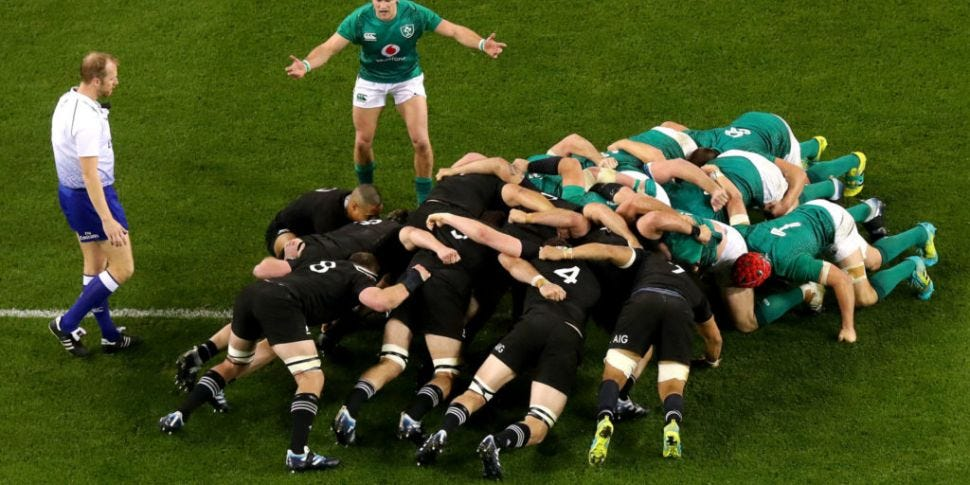
\includegraphics[width=0.8\linewidth]{scrum.jpg}
				\caption{Scrum formation}
			\end{figure}
		\end{column}
	\end{columns}

\end{frame}

%------------------------------------------------

\section{The functionning of the Scrum Methodology}
\subsubsection{Scrum Events}
\subsubsection{Scrum Artifacts}
\subsubsection{Scrum Process}

\begin{frame}
	\frametitle{Generally} 
	The framework involves breaking down projects into iterations, 
	known as sprints,  a sprint can have a duration 
	that generally varies between two weeks and a month.
\end{frame}


\begin{frame}
	\frametitle{Scrum events}
	The Sprint is a container for all other
	events. Each event in Scrum is a formal
	opportunity to inspect and adapt Scrum 
	artifacts. These events are specifically
	designed to enable the transparency required
	\begin{columns}[c] % The "c" option specifies centered vertical alignment while the "t" option is used for top vertical alignment
		\begin{column}{0.4\textwidth} % Left column width
			\begin{itemize} % Left column width
				\item Sprint
				\item Sprint Plaining
				\item Daily Scrum
				\item Sprint Review
				\item Sprint Retrospective
			\end{itemize}
		\end{column}
		\begin{column}{0.7\textwidth} % Right column width
			\begin{figure}
				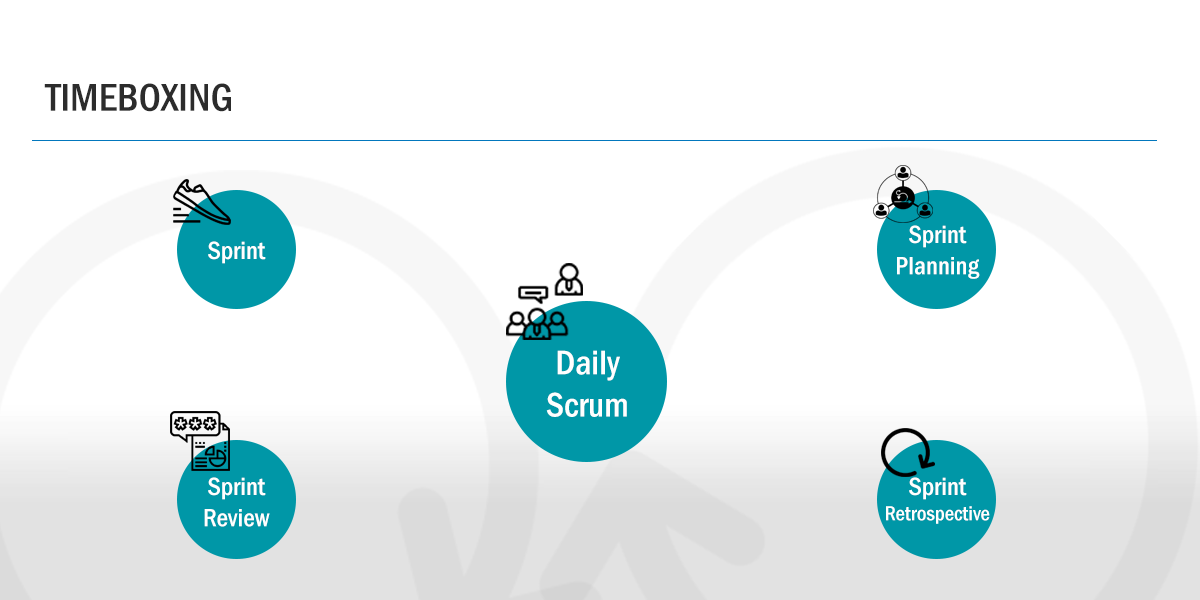
\includegraphics[width=1\linewidth]{events.png}
				\caption{Scrum events}
			\end{figure}
		\end{column}
	\end{columns}
\end{frame}






\begin{frame}
	\frametitle{Scrum artifacts}
	Scrum's artifacts represent work or value. 
	They are designed to maximize transparency
	of key information. Thus, everyone 
	inspecting them has the same basis for 
	adaptation
	\begin{columns}[c] % The "c" option specifies centered vertical alignment while the "t" option is used for top vertical alignment
		\begin{column}{0.4\textwidth} % Left column width
			\begin{itemize} % Left column width
				\item Product backlog
				\item Sprint backlog
				\item Product increment
			\end{itemize}
		\end{column}
		\begin{column}{0.7\textwidth} % Right column width
			\begin{figure}
				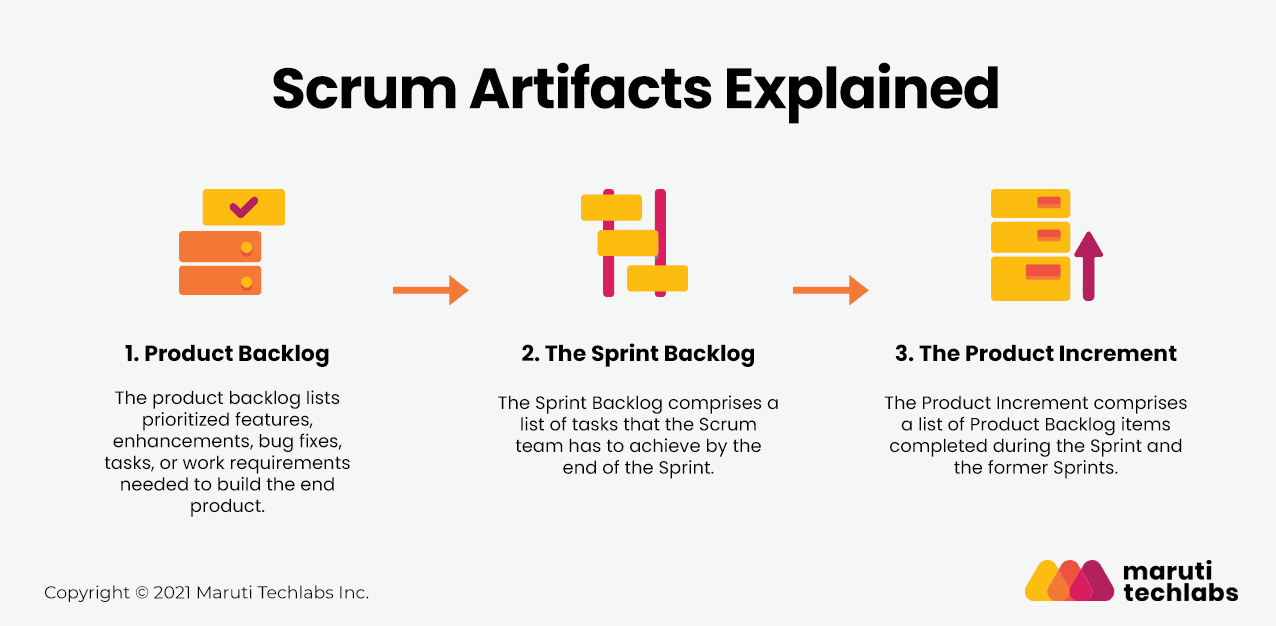
\includegraphics[width=0.8\linewidth]{Scrum_artifact.png}
				\caption{Scrum artifacts}
			\end{figure}
		\end{column}
	\end{columns}
\end{frame}


\begin{frame}
	\frametitle{Scrum process}
	\begin{figure}
	\centering
	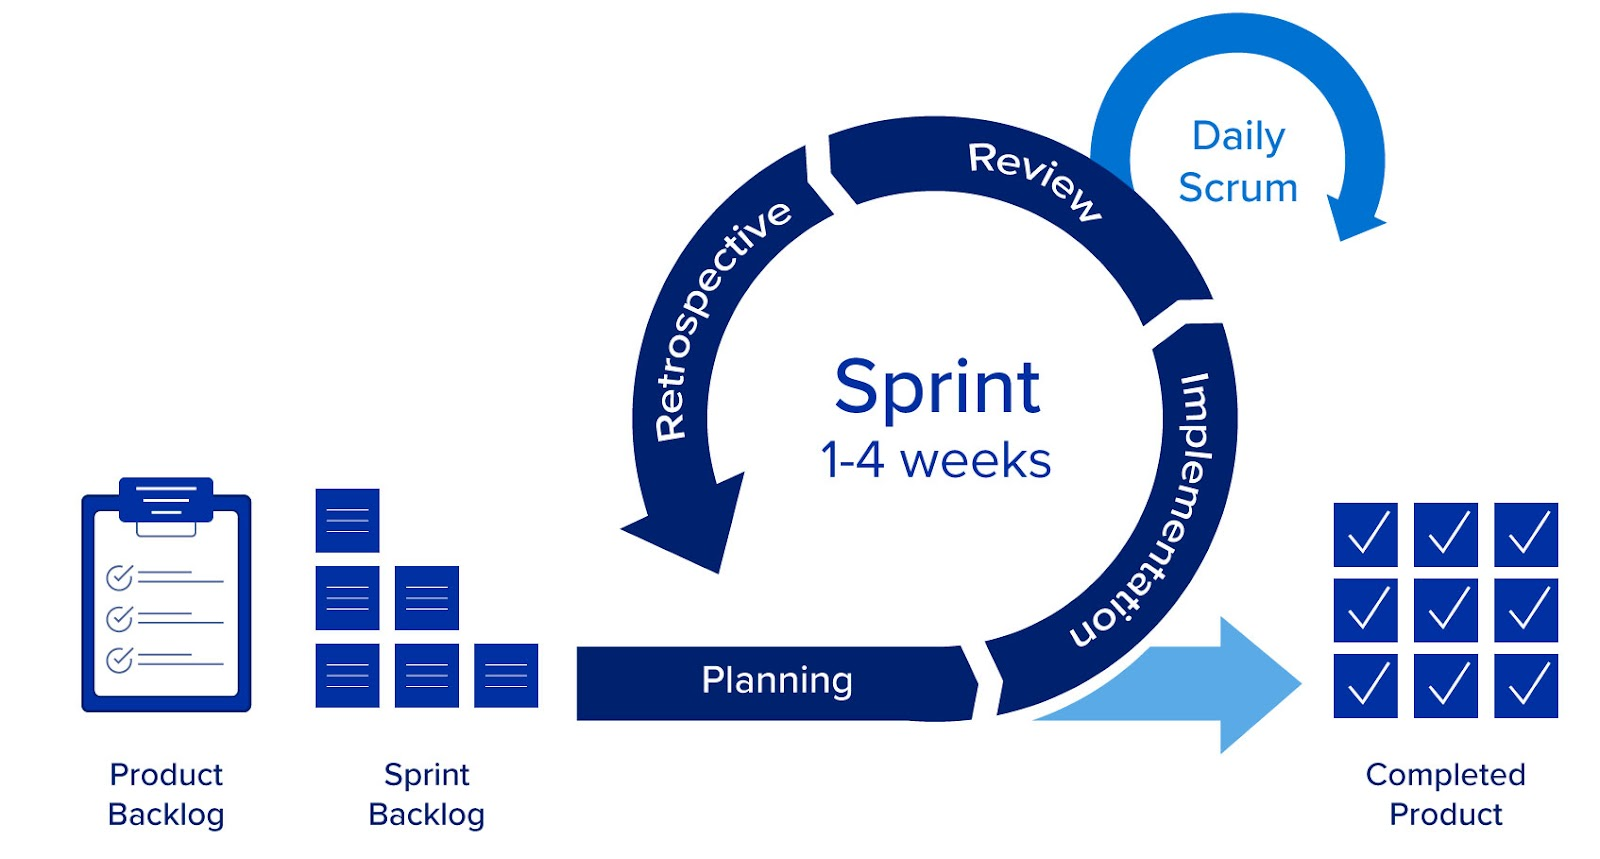
\includegraphics[width=0.8\textwidth]{fonc_Scrum.jpg}
	\caption{Scrum process}
	\end{figure}
	
\end{frame}



%------------------------------------------------  

\section{The Role and Principles of the Scrum Methodology}
\subsection{Role}
\subsection{Principles}

\begin{frame}
	\frametitle{The Role of the Scrum Methodology}
	We have 3 major roles for methods 
	\begin{itemize}
		\item Product Owner
		\item Scrum Master
		\item Development Team
	\end{itemize}
	\textbf{The product owner :} is the one who define the customer's needs and 
	vision for the final product. He work in collaboration with the rest of the team.
	\\
	\textbf{The Scrum Master:} his mission is to ensure that the team is fully operational and capable
	of accomplishing the tasks of each current sprint. He is a bridge between the product owner and the development team.
	\\
	\textbf{The Development Team:} is responsible for delivering the final 
	product at the end of each sprint.
\end{frame}

\begin{frame}
	\frametitle{The Role of the Scrum Methodology}
	\begin{figure}
		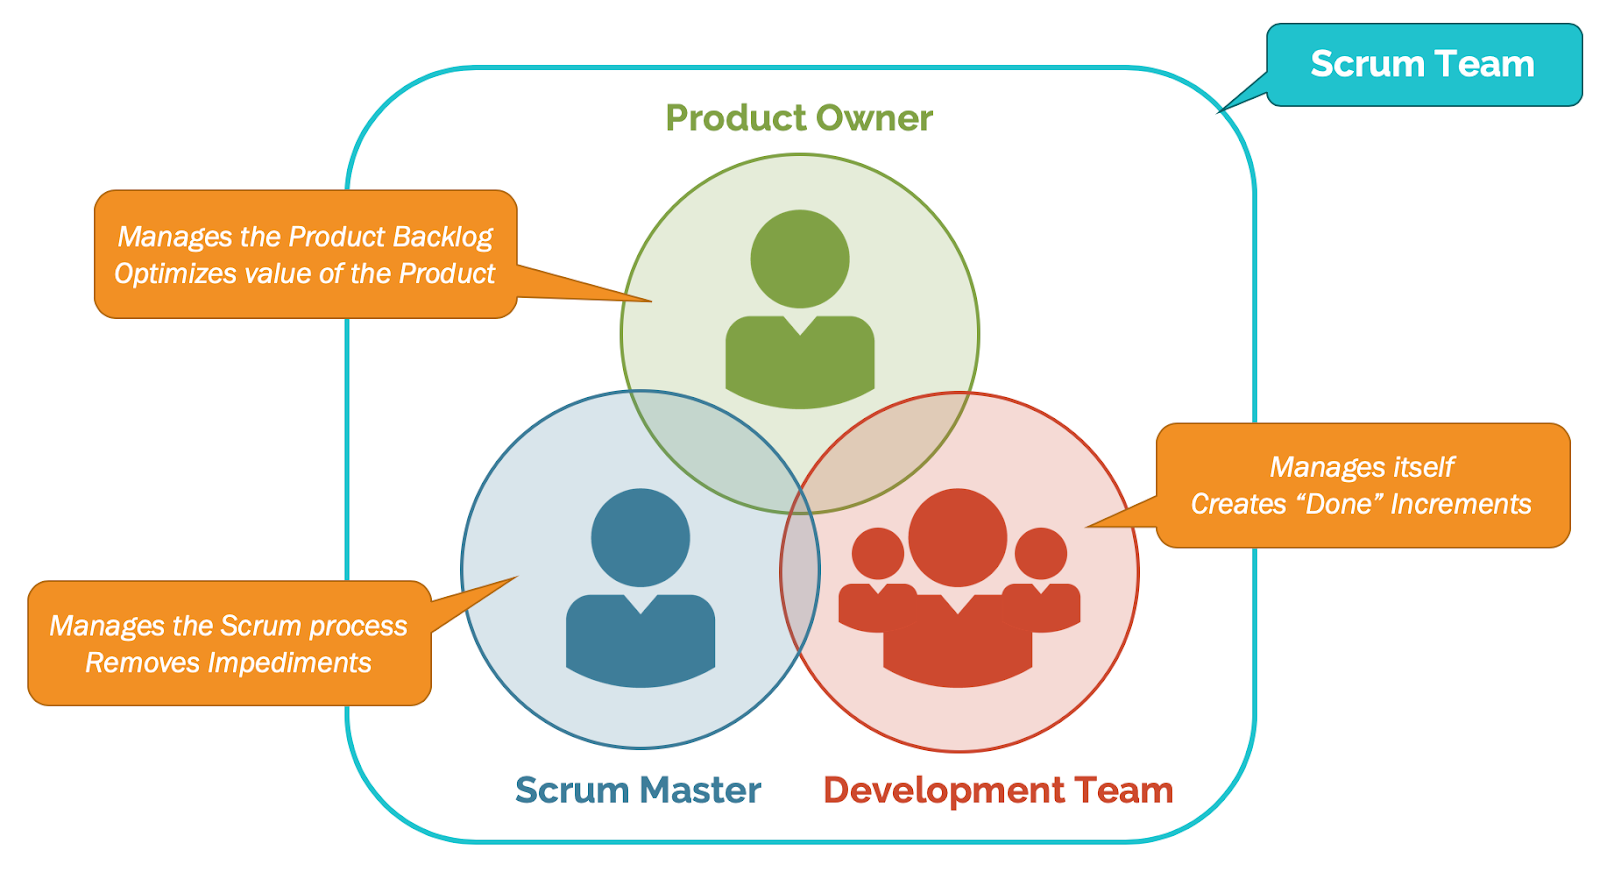
\includegraphics[width=0.8\linewidth]{Role.png}
		\caption{Scrum roles.}
	\end{figure}
\end{frame}

%------------------------------------------------

\begin{frame}
	\frametitle{The principles}
	The Scrum Method is based on six principles that enable the 
	A team that using it to be more efficient and productive.
	the principles are  
	\begin{itemize}
		\item Empirical Process Control
		\item Self-organization
		\item Collaboration
		\item Value-based Prioritization
		\item Time-boxing
		\item Iterative Development
	\end{itemize}
\end{frame}

\begin{frame}
	\frametitle{The Principles of the Scrum Methodology}
	\begin{figure}
		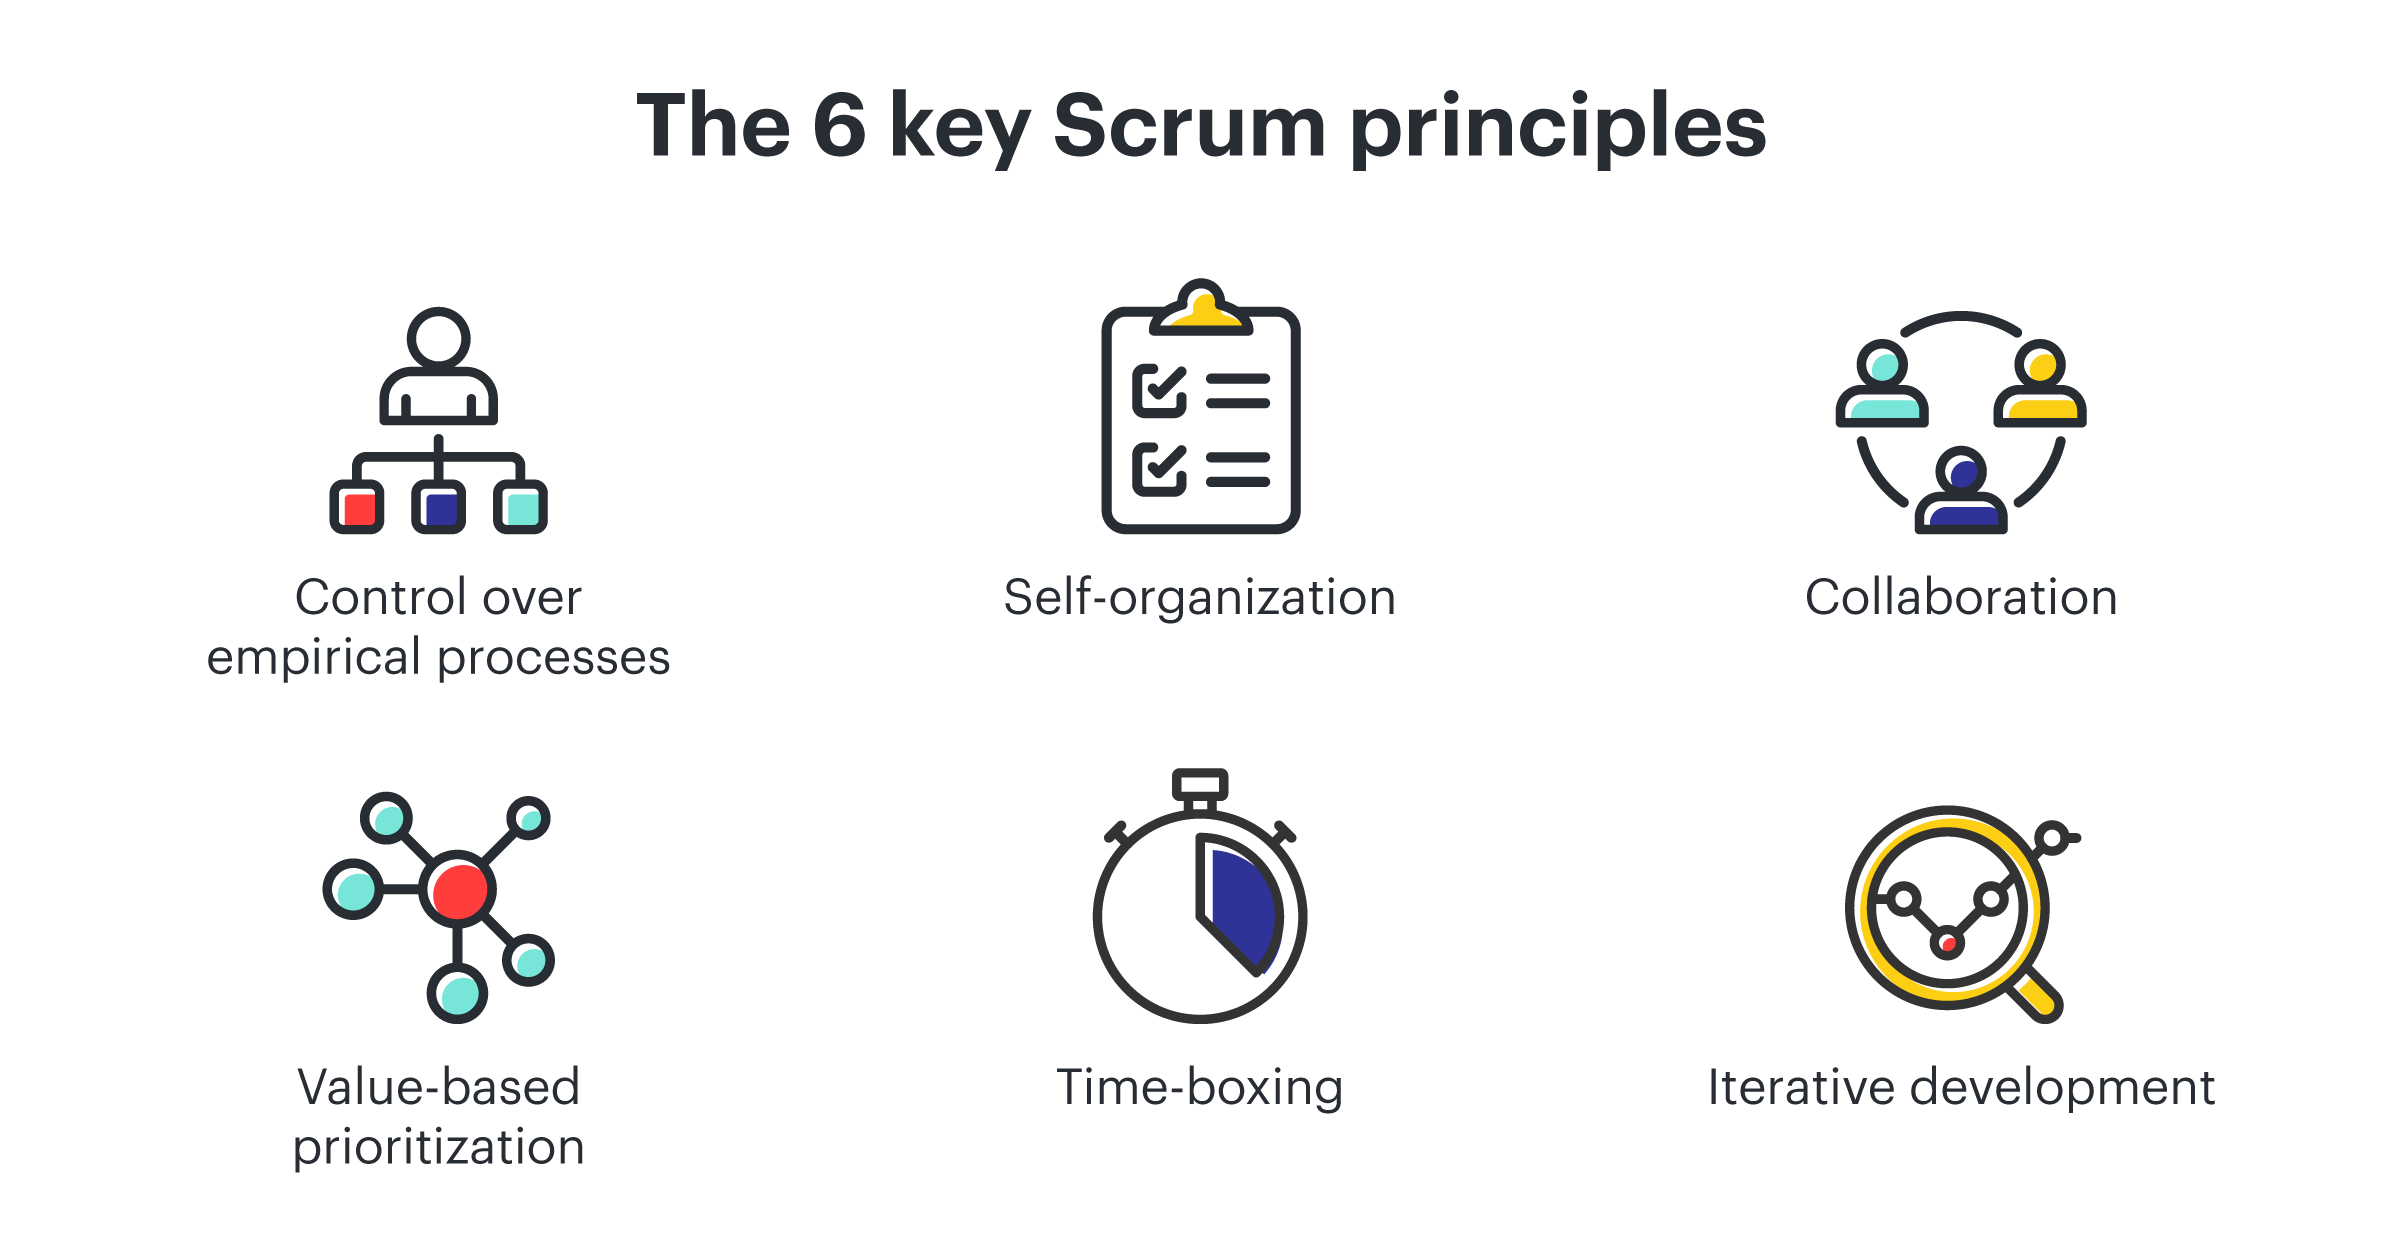
\includegraphics[width=0.8\linewidth]{principles.png}
		\caption{Scrum principles.}
	\end{figure}
\end{frame}

% 
%------------------------------------------------



\section{avantages and disadvantages of the Scrum Methodology}
\subsection*{Advantages of scrum}
\begin{frame}
	\frametitle{Advantages and disadvantages}
	\begin{itemize} 
		\item Adaptability and flexibility.
		\item Creativity and innovation.
		\item Time to market
		\item Lower Costs.
		\item Creates Transparency.
	\end{itemize}
\end{frame}

\subsection*{Advantages of scrum}
\begin{frame}
	\frametitle{Advantages and disadvantages}

	The text of the one who will present this part
\end{frame}



\section{Conclusion}
\subsection{conclusion}

\begin{frame}
	\frametitle{Conclusion}
	Scrum is a simple, lightweight, and adaptable framework that 
	teams can employ to continuously deliver value throughout a project.
	Scrum offers an excellent way of structuring work, with many advantages.
	It aims to create working environments where people are productive and happy.
	Besides, it provides a perfect approach for managing complex projects.
\end{frame}

%------------------------------------------------
\section{References}

\begin{frame}[allowframebreaks] % Use [allowframebreaks] to allow automatic splitting across slides if the content is too long
	\begin{thebibliography}{91}
		\bibitem{schwaber2021scrum}Schwaber, K. \& Sutherland, J. The Scrum Guide. 2020. {\em Accessed April}. (2021)
        \bibitem{sutherland1995scrum}Sutherland, J. \& Schwaber, K. The SCRUM methodology. {\em Business Object Design And Implementation: OOPSLA Workshop}. (1995)
		\bibitem{Carvalho}Carvalho, Henrique, Pereira Mello, Scrum agile product development 
		method -literature revie, analysis and classification (2011)
		\bibitem{Scrumstudy} www.scrumstudy.com, Scrum Principles, (2024)
	\end{thebibliography}
\end{frame}


%----------------------------------------------------------------------------------------
%	CLOSING SLIDE
%----------------------------------------------------------------------------------------

\begin{frame}[plain] % The optional argument 'plain' hides the headline and footline
	\begin{center}
		{\Huge The End}

		\bigskip\bigskip % Vertical whitespace

		{\LARGE Questions? Comments?}
	\end{center}
\end{frame}

%----------------------------------------------------------------------------------------

\end{document}